%! Author = Dean
%! Date = 12/28/2023

\chapter{Evolucija konvolucijskih neuronskih mreža}\label{ch:evolucija-konvolucijskih-neuronskih-mreza}
Konvolucijske neuronske mreže \emph{KNM} predstavlja ključnu inovaciju u području analize slika i obrade vizualnih podataka.
U posljednjem razdoblju, KNM arhitektura doživjela je značajan tehnološki napredak.
Ovaj napredak omogućio je postizanje rezultata koji su prije bili nezamislivi, često se približavajući ili čak nadmašujući ljudske sposobnosti u određenim zadacima vizualne analize.
Današnje vrijeme karakterizira raznolikost KNM-ova, s različitim arhitekturama koje su prilagođene specifičnim zadatcima.
Svaka arhitektura ima svoje prednosti i mane, a \enquote{Teorem besplatnog ručka} ukazuje na to da nema univerzalno najbolje arhitekture.

\section{Neocognitron}\label{sec:neocognitron}
Možemo reći da je Neocognitron preteča konvolucijskih neuronskih mreža.
Ova arhitektura je prva uvela pojmove kao što su ekstrakcija značajki (\emph{feature extraction}), konvolucija (\emph{convolution}), i slojevi uzorkovanja (\emph{pooling layers}).
\FloatBarrier
\begin{figure}[h]
    \centering
    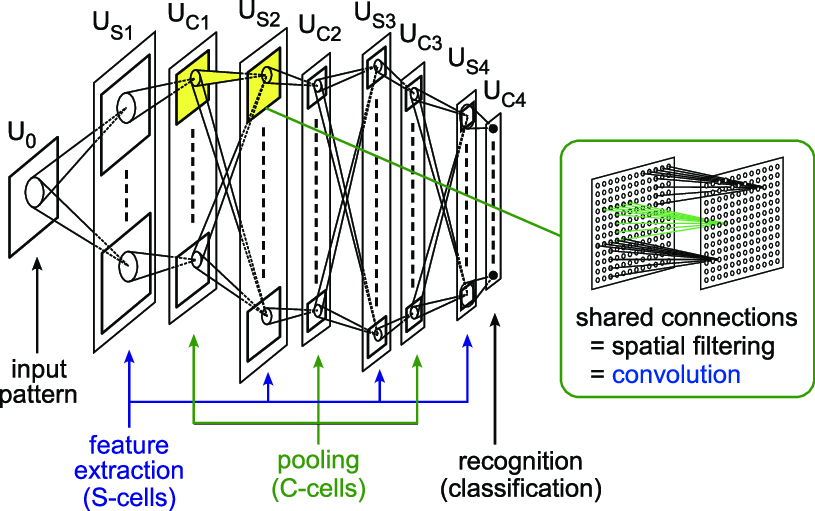
\includegraphics[width=0.6\textwidth]{images/Neocognitron}
    \caption{Arhitektura Neocognitron
    \protect\footnotemark}
    \label{fig:slika7}
\end{figure}
\FloatBarrier
\footnotetext{\url{https://www.researchgate.net/figure/The-architecture-of-the-neocognitron_fig1_336163445}}
Arhitektura Neocognitrona sastoji se od alternirajućih S i C slojeva, pri čemu svaki od njih sadrži S i C stanice.
S stanice, ili jednostavne stanice, služe za detekciju lokalnih značajki, dok C stanice, ili kompleksne stanice, služe za dodavanje tolerancije prema samoj poziciji objekta.
Na taj način dobivamo model koji je invarijantan na translacijske promjene, odnosno trebao bi prepoznati oblik bez obzira na to gdje se nalazi na slici.

\section{LeNet-5}\label{sec:lenet-5}
LeNet-5 je dizajnirana od strane francuskog informatičara Yanna LeCuna između 1989. i 1998. godine i postigla je uspjeh u prepoznavanju rukom pisanih brojeva.

Arhitektura se sastojala od tri konvolucijska sloja i dva sloja za uzrokovanje koji su bili međusobno alternirajući. Na kraju su se nalazila dva potpuno povezana sloja.

U konvolucijskim slojevima koristio se 5x5 filter s korakom veličine 1, odnosno s pomakom veličine 1. S druge strane, slojevi za uzrokovanje bili su 2x2 s pomakom veličine 2.
\begin{figure}[h]
    \centering
    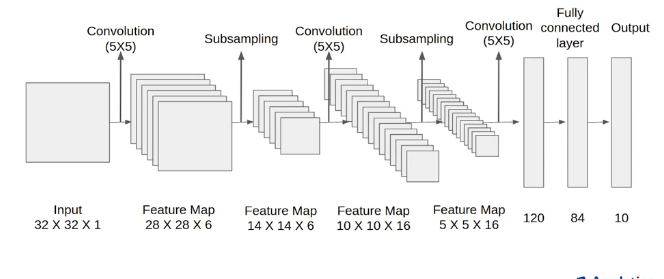
\includegraphics[width=0.6\textwidth]{images/LeNet}
    \caption{Arhitektura LeNet-5.
    \protect\footnotemark}
    \label{fig:slika8}
\end{figure}
\footnotetext{\url{https://www.analyticsvidhya.com/blog/2021/03/the-architecture-of-lenet-5/}}

Dimenzija ulazne slike je 32x32x1 jer se ova arhitektura uglavnom koristila za prepoznavanje rukom pisanih brojeva. Dimenzije označavaju širinu, visinu i dubinu slike. Za crno-bijele slike dubina je 1, što znači da postoji samo jedan kanal. Za RGB slike, dubina bi bila 3 (jedan kanal za crvenu, zelenu i plavu komponentu svake boje).

Prvi konvolucijski sloj ima 6 filtera veličine 5x5 s pomakom od 1.
Rezultat tog sloja je značajka veličine 28x28x6.
Izlazni sloj se može izračunati pomoću formule: \[ \textit{dimenzija} = \frac{\textit{ulazna dimenzija} - \textit{veličina filtera}}{\textit{korak}} + 1 \].

Nakon toga slijedi sloj za uzrokovanje veličine 2x2.
Ovdje se koristi average pooling koji za vrijednost uzima prosjek od odabrane 4 vrijednosti.

Dalje slijede još dva konvolucijska sloja, jedan sloj za uzrokovanje i dva potpuno povezana sloja, od kojih je jedan izlazni sloj.
Izlazni sloj sastoji se od 10 neurona i koristi Softmax kao aktivacijsku funkciju.
Softmax je prikladan jer za svaku klasu daje vjerojatnost da ulaz pripada toj klasi, a predikcija se izvodi tako da se odabere klasa s najvećom vjerojatnošću.

\section{AlexNet}\label{sec:alexnet}
AlexNet je arhitektura konvolucijske neuronske mreže koja se primarno koristi za klasifikaciju slika. Koristi 5 konvolucijskih slojeva u kombinaciji s max poolingom, a na kraju ima 3 potpuno povezana sloja. Kao aktivacijsku funkciju koristi ReLU, osim na izlaznom sloju gdje se i dalje koristi Softmax. Primjenom ReLU aktivacije uspjeli su ubrzati proces treniranja čak 6 puta.

Za razliku od LeNet-5 modela, ulaz u AlexNet je RGB slika dimenzija 227x227.
\FloatBarrier
\begin{figure}[h]
    \centering
    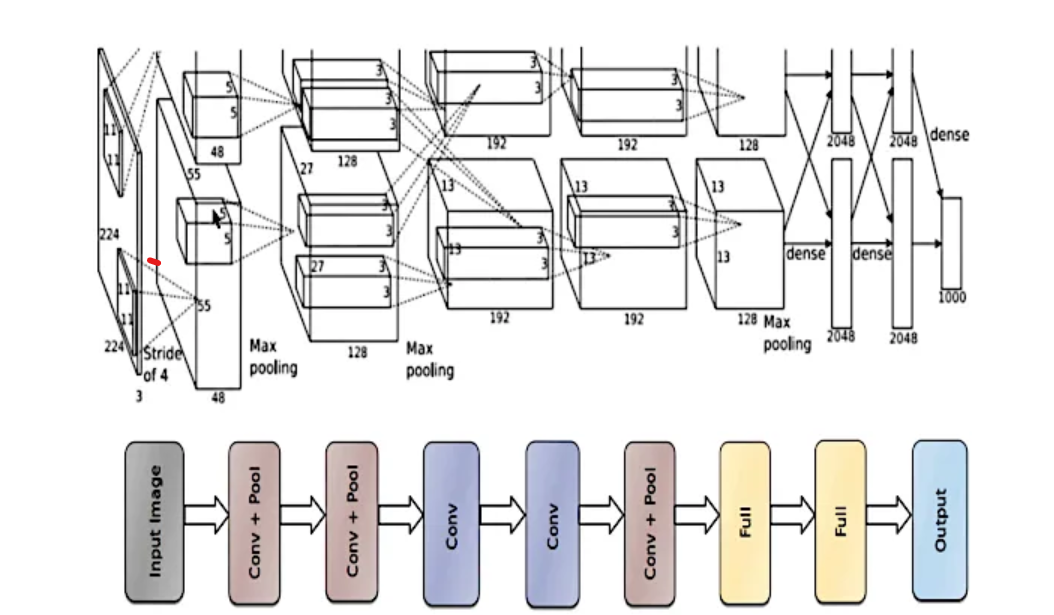
\includegraphics[width=0.6\textwidth]{images/AlexNet}
    \caption{Arhitektura AlexNet
    \protect\footnotemark}
    \label{fig:slika9}
\end{figure}
\FloatBarrier
\footnotetext{\url{https://www.analyticsvidhya.com/blog/2021/03/introduction-to-the-architecture-of-alexnet/}}


Ako se pogleda arhitektura, primjećuje se da se broj filtera povećava kako dublje ide u mrežu, što znači da se može izvući više značajki.
Također, veličina filtra se smanjuje kako dublje ulazimo u mrežu.
Mreža se sastoji od 62.3 miliona parametara, za usporedbu LeNet-5 ima 60000.
Zbog ogromne količine parametara, moramo paziti da nam model ne postane prenaučen te se u tu svrhu koristi regularizacija.
Kod AlexNet-a za regularizaciju se koristi takozvani dropout.
Ideja dropout-a je jednostovna: tijekom treninga, nasumično se \enquot{isključuju} određeni neuroni u mreži i ona su privremena i mijenjaju se u svakoj iteraciji treninga.
Samim time što tijekom treninga mi isključimo jedan dio neurona, dovodi mrežu u situaciju da smanjuje međuovisnost o neuronima, da se prilagodi različitim kombinacijama neurona koji su prisutni.
Kao uvijek postoje i šumovi u podatcima, a pomoću dropout-a sprečava se memorizacija šumova što pomaže da model bolje generalizira.
Naravno tijekom testiranja dropout se ne radi.

\section{VGGNet}\label{sec:vggnet}
VGGNet arhitektura je razvijena od strane Visual Geometry Group na Sveučilištu Oxford.
Grupa je radila s pretpostavkom da dublje strukture konvolucijskih mreža mogu bolje modelirati nelinearnosti.

\FloatBarrier
\begin{figure}[h]
    \centering
    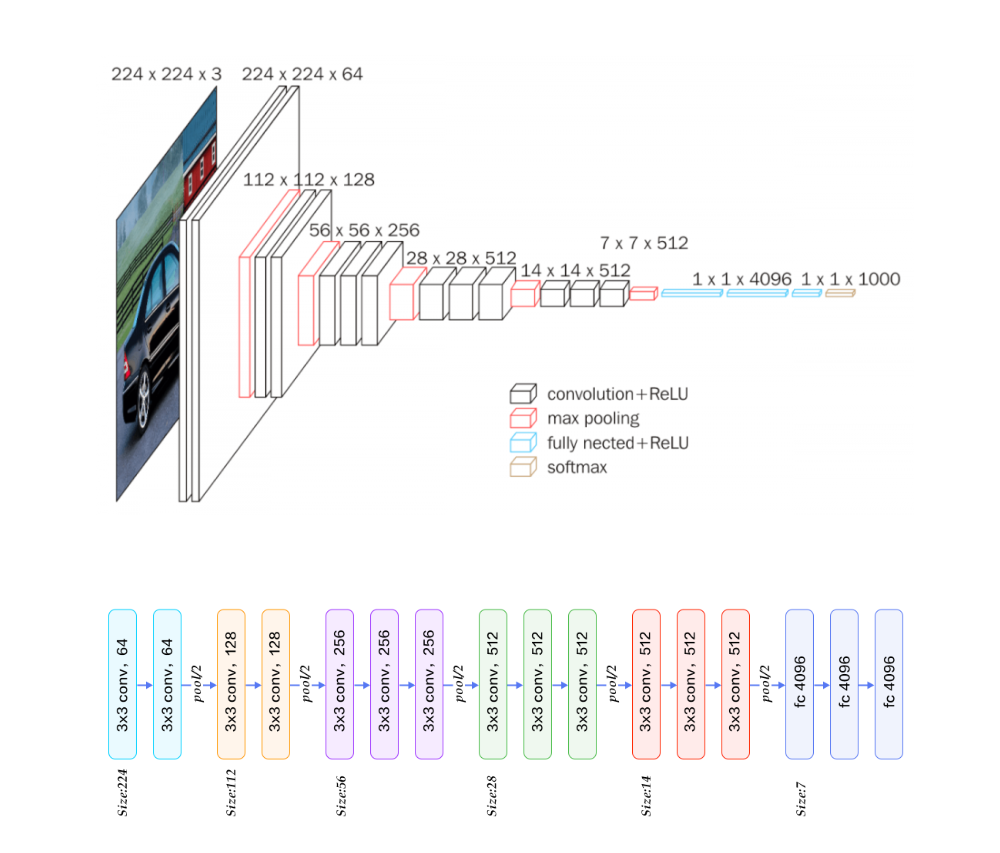
\includegraphics[width=0.6\textwidth]{images/VGGNet}
    \caption{Arhitektura VGGNet
    \protect\footnotemark}
    \label{fig:slika10}
\end{figure}
\FloatBarrier
\footnotetext{\url{https://www.kaggle.com/code/blurredmachine/vggnet-16-architecture-a-complete-guide}}
Ulaz u mrežu je RGB slika dimenzija 224x224.
Modeli čija se dubina razlikuje u rasponu od VGG11 do VGG19 imaju različite strukture, pri čemu je VGG11 sastavljen od 8 konvolucijskih slojeva i 3 potpuno povezana sloja, dok VGG19 ima 16 konvolucijskih slojeva i 3 potpuno povezana sloja.
Kako bi se smanjio broj parametara, odlučeno je postaviti veličinu filtra na 3x3 za svaki sloj u mreži.
Ali i sa tom modifikacijom model će imati ogroman broj parametara.
Recimo VGG16 će u konačnici imati 138357544 parametara.
Za treniranje se koristi gradijentni spust s momentom \emph{0.9}.
Kao regularizaciju koristi L2 regularizaciju i dropout koji se koristi nakon drugog potpuno povezanog sloja s vrijednosti od 50\%.

\section{GoogLeNet}\label{sec:googlenet}
GoogLeNet je razvijena od strane Googla i oni su se fokusirali na arhitekturi koja ima što veću dubinu, baš kao što je radila Visual Geometry Group s VGGNet-om.
Ali za razliku od prethodnika, dodantan fokus je bio na smanjenju parametara i boljoj memorijskoj efikasnosti
Ovaj model broji do 22 sloja, ali ovaj model uopće nema potpuno povezane slojeve što je drastično smanjilo broj parametara, točnije na 5 miliona.

\FloatBarrier
\begin{figure}[h]
    \centering
    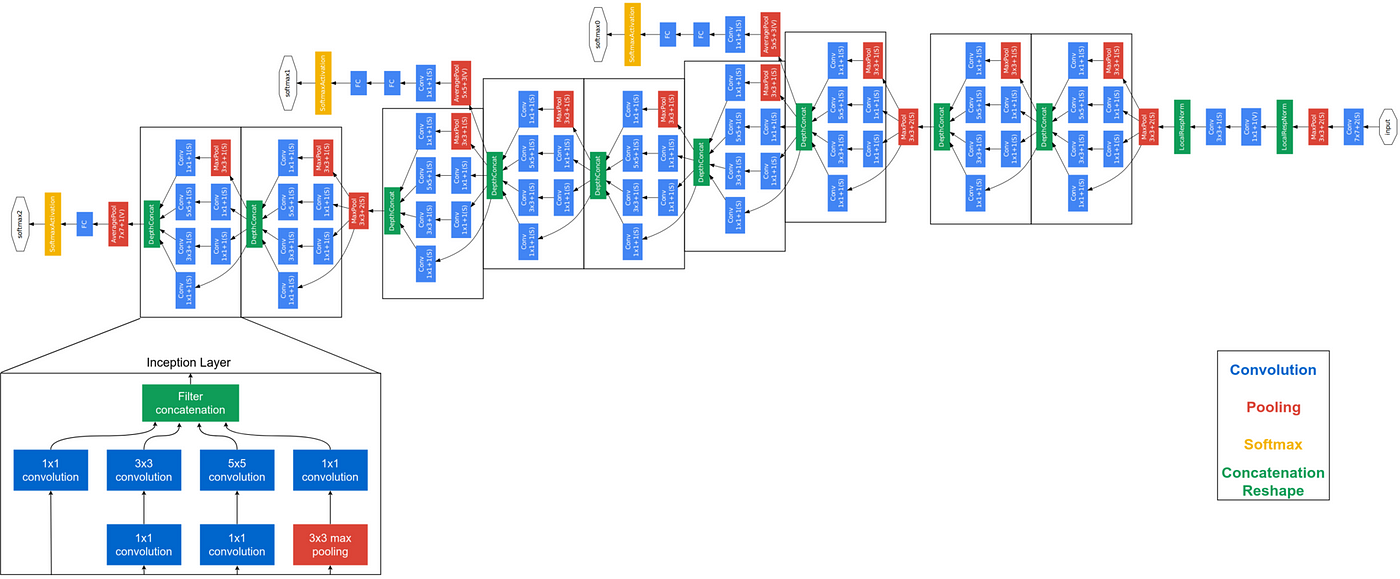
\includegraphics[width=0.6\textwidth]{images/GoogLeNet}
    \caption{Arhitektura GoogleLeNet
    \protect\footnotemark}
    \label{fig:slika11}
\end{figure}
\FloatBarrier
\footnotetext{\url{https://ai.plainenglish.io/googlenet-inceptionv1-with-tensorflow-9e7f3a161e87}}

Ključna inovacija za ovaj uspjeh je bio inception model koji se koristi više puta kroz mrežu.
Glavna ideja iza inception modela je da ne biramo mi da li ćemo koristit konvoluciju 1x1 ili 3x3 ili 5x5 ili ćemo možda koristiti max pooling, nego koristimo sve to zajedno i na kraju konkateniramo rezultat.
Naravno nije sve idealno, pa tako i ovaj način ima nedostataka.
Glavni nedostatak je taj što je računski dosta zahtjevno jer traži puno operacija za bi se obradio jedan inception sloj.
Ali kako bi se smanjio broj operacija koji se mora izvesti unutar jednog inception sloja, onda se prvo provuče kroz konvoluciju 1x1 a tek onda na konvolucije 3x3 ili 5x5.

\FloatBarrier
\begin{figure}[h]
    \centering
    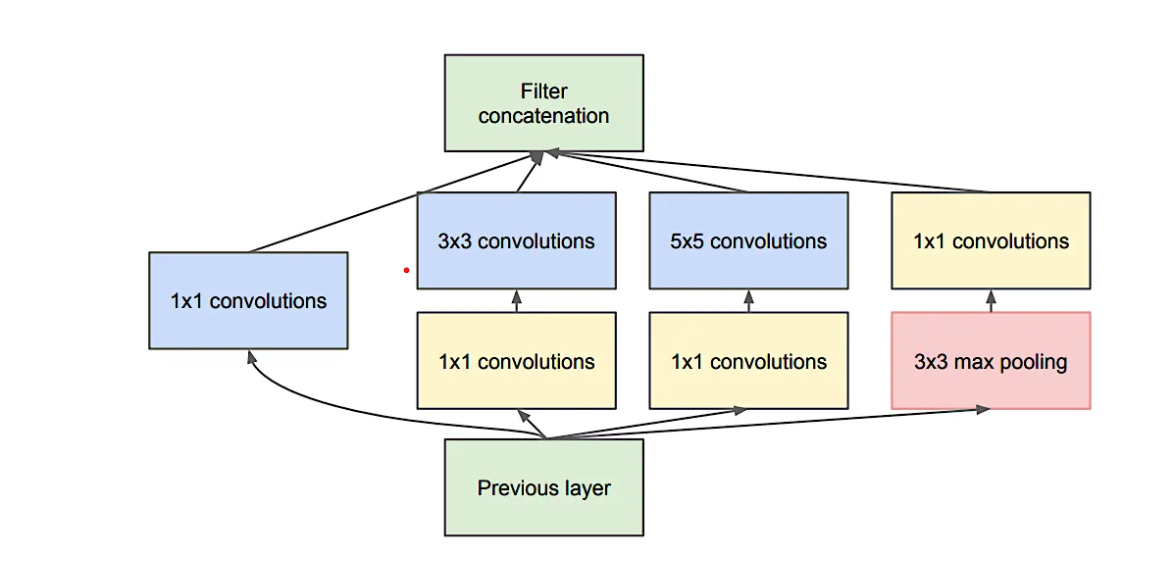
\includegraphics[width=0.4\textwidth]{images/Inception}
    \caption{Inception model
    \protect\footnotemark}
    \label{fig:slika12}
\end{figure}
\FloatBarrier
\footnotetext{\url{https://ai.plainenglish.io/googlenet-inceptionv1-with-tensorflow-9e7f3a161e87}}
